\subsection{Reward Ablation}
\label{sec:eval:beta}
\begin{figure*}[!t]
\centering
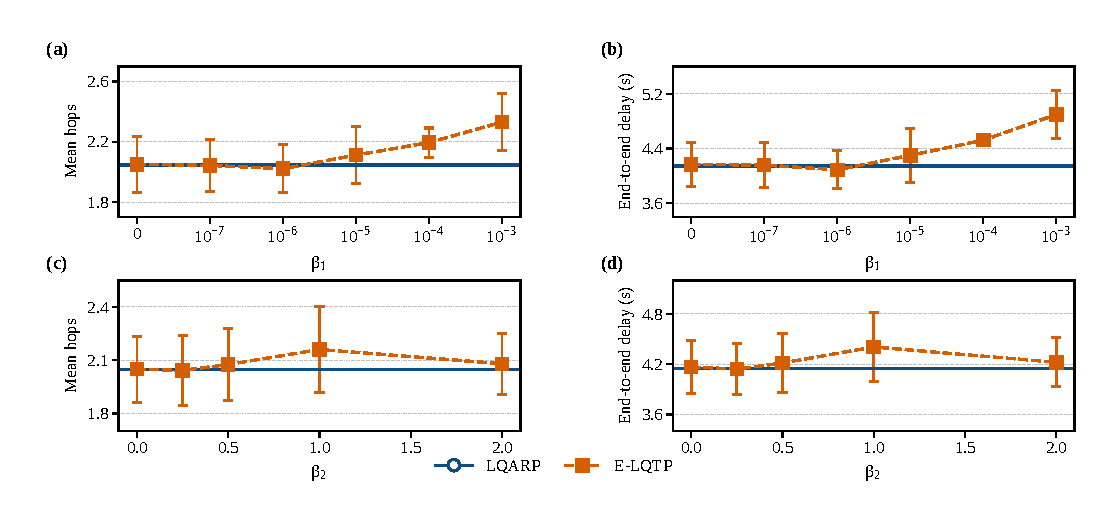
\includegraphics[width=\textwidth]{elqtp_figs/fig6_reward_ablation}
\caption{Scenario~III reward sweep. Solid line: LQARP. Error bars
are the five-seed sample standard deviation. No tested $\beta$
improves hops or delay.}
\label{fig:reward_ablation}
\end{figure*}

Table~\ref{tab:beta_sweep} and Fig.~\ref{fig:reward_ablation} sweep
$\beta_1$ at $\beta_2=0$ and $\beta_2$ at $\beta_1=0$ on
Scenario~III.
At $\beta_1=10^{-6}$ mean hops fall to $2.021\pm 0.158$ against
LQARP's $2.046\pm 0.187$ ($0.988\times$); that dip sits inside
LQARP's between-seed band and is not read as a routing gain.
Once $\beta_1$ leaves the blend-scale range, hops, delay, and
energy rise together, reaching $1.14\times$ hops and
$1.18\times$ delay at $\beta_1=10^{-3}$.
The $\beta_2$ column stays within $0.998\times$--$1.056\times$
LQARP hops with no monotonic trend.
No tested weight improves hops, delay, or energy relative to
LQARP's between-seed band.
A Scenario~II-specific $\beta_2$ sweep against the sustained
AUV--sink range-rate of uniform drift remains future work.
The validated operating point is therefore $\beta_1=\beta_2=0$:
the control-plane gain is the event trigger, and the reward
modifiers are a documented negative result.

% Scenario III reward sweep. Five columns: single-column table.

\begin{table}[!t]
\caption{Scenario~III $\beta$ sweeps (five seeds). No tested weight
beats LQARP's hop or delay band.}
\label{tab:beta_sweep}
\centering
\scriptsize
\resizebox{\columnwidth}{!}{%
\begin{tabular}{lcccc}
\hline
Weight & PDR & $T_{\mathrm{e2e}}$ (s) & $E_{\mathrm{bit}}$ & Hops \\
\hline
LQARP & $0.9989\pm 0.0018$ & $4.146\pm 0.348$ & $1.099\pm 0.098\times 10^{-2}$ & $2.046\pm 0.187$ \\
\hline
\multicolumn{5}{l}{$\beta_1$ sweep ($\beta_2=0$)} \\
$0$ & $0.9989\pm 0.0018$ & $4.167\pm 0.318$ & $1.101\pm 0.097\times 10^{-2}$ & $2.050\pm 0.186$ \\
$10^{-7}$ & $0.9986\pm 0.0017$ & $4.159\pm 0.324$ & $1.098\pm 0.092\times 10^{-2}$ & $2.043\pm 0.175$ \\
$10^{-6}$ & $1.0000\pm 0$ & $4.090\pm 0.279$ & $1.083\pm 0.085\times 10^{-2}$ & $2.021\pm 0.158$ \\
$10^{-5}$ & $1.0000\pm 0$ & $4.301\pm 0.399$ & $1.132\pm 0.103\times 10^{-2}$ & $2.111\pm 0.192$ \\
$10^{-4}$ & $0.9976\pm 0.0040$ & $4.523\pm 0.082$ & $1.185\pm 0.056\times 10^{-2}$ & $2.194\pm 0.097$ \\
$10^{-3}$ & $0.9980\pm 0.0027$ & $4.897\pm 0.351$ & $1.253\pm 0.099\times 10^{-2}$ & $2.330\pm 0.188$ \\
\hline
\multicolumn{5}{l}{$\beta_2$ sweep ($\beta_1=0$)} \\
$0$ & $0.9989\pm 0.0018$ & $4.167\pm 0.318$ & $1.101\pm 0.097\times 10^{-2}$ & $2.050\pm 0.186$ \\
$0.25$ & $0.9989\pm 0.0018$ & $4.140\pm 0.304$ & $1.097\pm 0.103\times 10^{-2}$ & $2.042\pm 0.197$ \\
$0.50$ & $0.9989\pm 0.0018$ & $4.214\pm 0.349$ & $1.115\pm 0.106\times 10^{-2}$ & $2.076\pm 0.204$ \\
$1.00$ & $0.9989\pm 0.0018$ & $4.405\pm 0.415$ & $1.160\pm 0.126\times 10^{-2}$ & $2.161\pm 0.240$ \\
$2.00$ & $0.9989\pm 0.0018$ & $4.221\pm 0.293$ & $1.117\pm 0.090\times 10^{-2}$ & $2.080\pm 0.171$ \\
\hline
\end{tabular}}
\end{table}

